\section{Analisi Dati e Velocità}
\label{Analisi Dati e Velocità}



\subsection{Lettura dati}

Si considera il segnale osservato dal ricevitore a 1,4 GHz e lo si grafica in funzione della frequenza:

\begin{figure}[H]
	\centering
	\includegraphics[scale=0.8]{Segnale_colorato.pdf}
	\caption{Segnale misurato, ogni colore rappresenta uno dei 150 record. L'immagine ivi presente, come le successive, sono riferite a un campionamento svolto in data 05/03/2023}
    	\label{fig:Segnale_colorato}
\end{figure}

Ogni colore rapprsenta i dati di un particolare record. Di conseguenza, il grafico ottenuto è costituito da 150 colori differenti. Le intensità dei record sono molto simili l'una con l'altra.
Il segnale graficato è espresso in scala logaritmica, si passa quindi alla scala lineare convertendo i valori da dBmW a mw. Viene fatta, poi, una media del segnale lineare sui 150 record.
\\\\
Successivamente, si restringe lo studio del segnale nell'intorno della regione della riga H 21 e si osserva che si hanno tre picchi relativi a quest'ultima. Questo è dovuto alla presenza di tre regioni di idrogeno distinte che si muovono a velocità differenti.

\begin{figure}[H]
	\centering
	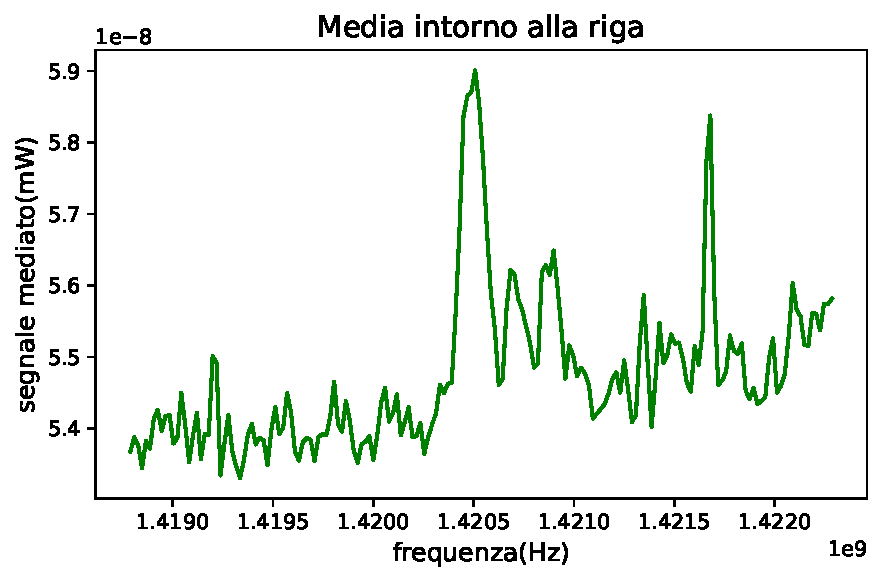
\includegraphics[scale=0.8]{Media_segnale.pdf}
	\caption{Segnale dopo aver eseguito la media mobile}
    	\label{fig:Media_segnale}
\end{figure}  

Si nota che il segnale risulta essere disturbato. Viene quindi eseguita una media mobile, mediando ciascun dato col precedente e col successivo.

\begin{figure}[H]
	\centering
	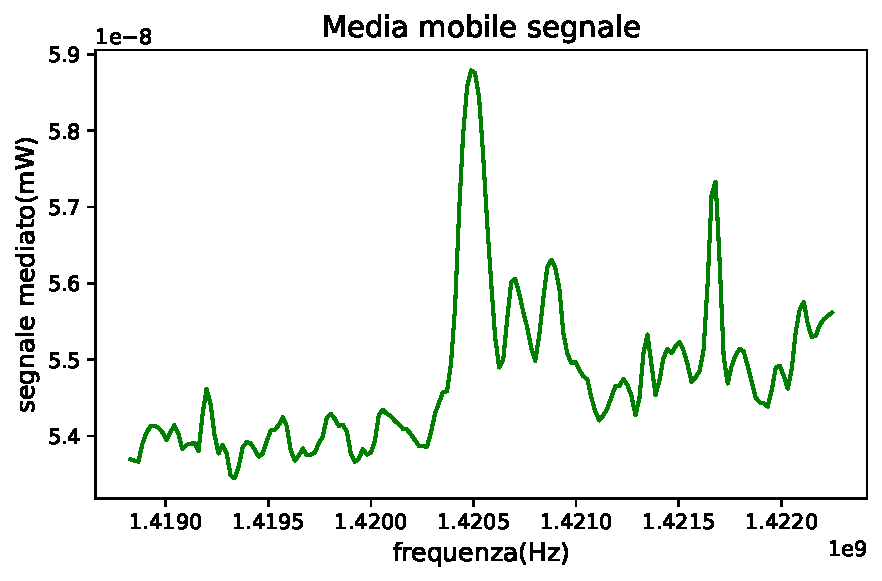
\includegraphics[scale=0.8]{Media_mobile_segnale.pdf}
	\caption{Segnale dopo aver eseguito la media mobile}
    	\label{fig:Media_mobile_segnale}
\end{figure}


\subsection{Temperatura di Brillanza}

Ora, si vuole calcolare la temperatura di brillanza $T_{B}$. Quest'ultima è una grandezza fondamentale nello studio di una sorgente astrofisica. Per ricavarla, possiamo utilizzare l'approssimazione $T_{B} \simeq T_{A}$, dove $T_{A}$ è la temperatura di antenna, poiché ci troviamo nel caso di sorgente estesa, $\Omega_{A} \ll \Omega_{B}$.\\
Per determinare $T_{A}$ utilizziamo la relazione:
\begin{equation}
    W_{out}=GT_{sys}=G[T_{A}+T_{room}]
\end{equation}
dove $G, T_{sys}$ e $T_{room}$ sono rispettivamente il Gain, la temperatura del sistema e la temperatura di rumore.
Da qui appunto si ottiene che:
\begin{equation}
    T_{A}=T_{sys}-T_{rum}=\frac{W_{out}}{G}-T_{room} 
\label{temp antenna}
\end{equation}
Nella temperatura ottenuta però, oltre al termine dovuto al segnale proveniente dal cielo, $T_{s}$, è contenuta anche la temperatura di rumore del cavo, $T_{c}$, secondo la relazione:
\begin{equation}
    T_{A}=T_{s}e^{-\tau}+T_{c}(1-e^{-\tau})
\end{equation}
Perciò, la temperatura di brillanza del solo segnale è data da:
\begin{equation}
    T_{s}=[T_{A}-T_{c}(1-e^{-\tau})]e^{\tau}
\label{temp cielo}
\end{equation}

\subsection{Sottrazione rumore}

Quindi, per prima cosa si converte il segnale in temperatura d'antenna utilizzando la relazione \eqref{temp antenna}.

\begin{figure}[H]
	\centering
	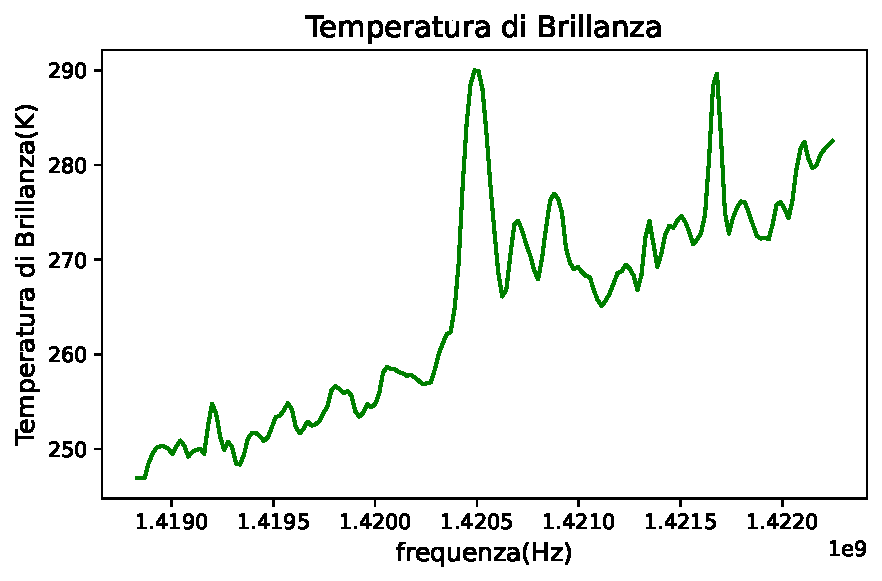
\includegraphics[scale=0.8]{Temperatura_brillanza_tutto.pdf}
	\caption{Grafico della temperatura complessiva di brillanza ( sorgente + contributo cavo + fondo del cielo}
    	\label{fig:Temperatura_brillanza_tutto}
\end{figure}

Successivamente si procede alla rimozione del segnale di fondo e della temperatura di rumore del cavo.\\
Per la rimozione del fondo si utilizza la libreria $Specutils$ di Python. Questa permette, tramite la funzione $fit\_continuum$, di fare un fit polinomiale del segnale escludendo determinate regioni. Nel nostro caso abbiamo escluso le regioni dei picchi che sovrastano il fondo. La funzione $fit\_continuum$, in particolare, per eseguire il fit, utilizza il Polinomio di Čebyšëv, la cui definizione in forma esplicita è data da:
\begin{equation}
    T_n(x)=\sum_{h=0}^{[n/2]} (-1)^h {n \choose 2h} x^{n-2h} (1-x^2)^h
\end{equation}
dove con $[n/2]$ si intende la parte intera di $n/2$. REFERENZA A WIKIPEDIA

\begin{figure}[H]
	\centering
	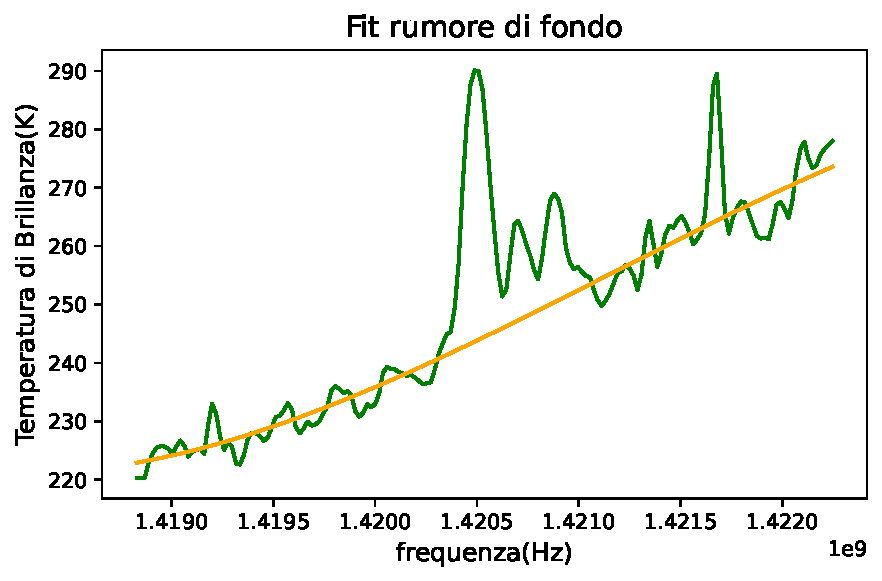
\includegraphics[scale=0.8]{Fit rumore di fondo.pdf}
	\caption{Sovrapposizione tra la temperatura di brillanza e il fit del solo fondo}
    	\label{fig:Fit rumore di fondo}
\end{figure}


Infine, per rimuovere la temperatura di rumore del cavo e ottenere quindi la temperatura di brillanza della sorgente si utilizza l'equazione \eqref{temp cielo}.

\begin{figure}[H]
	\centering
	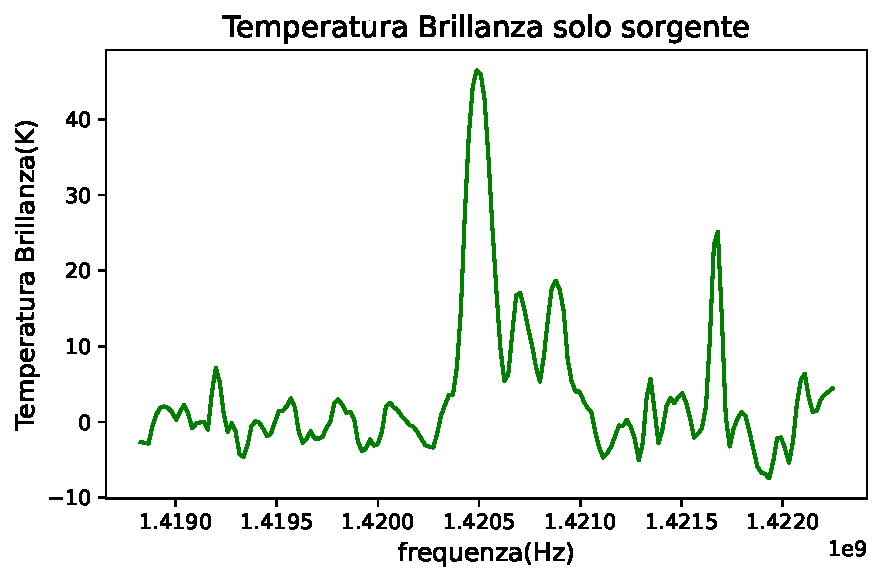
\includegraphics[scale=0.8]{Temperatura_finale.pdf}
	\caption{Temperatura di brillanza della sola sorgente}
    	\label{fig:Temperatura_finale}
\end{figure}

\subsection{Fit del segnale}

I picchi che osserviamo non sono delle Delta di Dirac, bensì presentano un allargamento dovuto a diversi fenomeni fisici. Inanzitutto, vi è l'allargamento naturale, dovuto al principio di indeterminazione di Heisemberg, per il quale $\Delta E\Delta t\geq\frac{\hbar}{2}$. Inoltre, è anche presente l'allargamento per collissioni, il quale si verifica quando atomi e molecole vengono in contatto con conseguente perturbazione dei loro livelli energetici. Questo dipende dalla loro configurazione elettronica e dalla velocità dell'urto. Infine, un altro tipo di fenomeno tipico è l'allargamento Doppler, causato da una distribuzione di velocità di atomi e molecole. Le diverse velocità delle particelle generano diversi Doppler shift, che sono la causa dell'argamento della riga.\\
Si effettua quindi un fit gaussiano di ciascun picco singolo e, in seguito, un fit multigaussiano dei tre picchi insieme.

\begin{figure}[H]
	\centering
	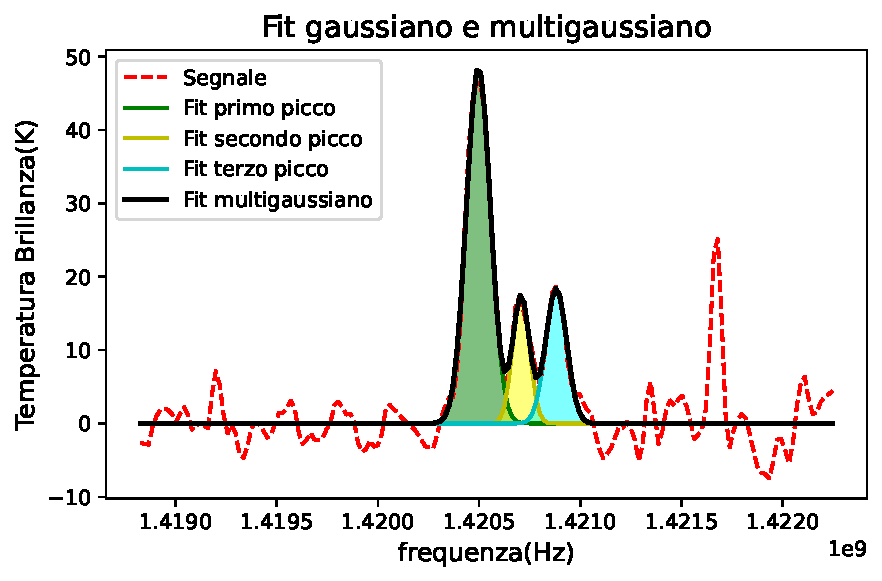
\includegraphics[scale=0.8]{Tre_picchi.pdf}
	\caption{Fit gaussiano e multigaussiano dei picchi}
    	\label{fig:Tre_picchi}
\end{figure}

CONSIDERAZIONE SUI FIT

\subsection{Calcolo delle velocità dei tre picchi}
\label{Calcolo delle velocità dei tre picchi}

Tramite l'effetto Doppler è possibile ricavare la velocità delle tre regioni di emissione. In particolare, l'effetto Doppler consiste nella variazione apparente della frequenza percepita da un osservatore, rispetto al valore vero della frequenza emessa da una sorgente in moto rispetto all'osservatore stesso. Vale quindi:

\begin{equation}
    f=\frac{c}{c\pm v}f_{0}
\end{equation}
Dove $f$ è la frequenza percepita dall'osservatore, $f_{0}$ è la frequenza della sorgente e $v$ è la velocità della sorgente. Al denominatore si usa il più quando la sorgente si allontana dall'osservatore, mentre si usa il meno quando si avvicina. Quest'ultimo è il nostro caso. Perciò la velocità delle tre regioni di emissione si ricava dalla legge:
\begin{equation}
    v=c (1-\frac{f_{0}}{f})
\end{equation}

Tramite il fit si ricava la frequenza dei tre picchi e quindi le velocità.


\subsection{Correzione col moto di rivoluzione terrestre}

\subsubsection{Correzione}

Prima di procedere con la misura della dispersione, è necessario applicare delle correzioni alle velocità ricavate. Viene presentata la descrizione della procedura generale, da effettuare per i set di velocità di ciascuno dei tre picchi.
\\\\
La necessità di applicare delle correzioni è intuibile dallo studio dell'andamento delle velocità in funzione del tempo, infatti i valori risultano aumentare al variare del giorno di osservazione. 

\begin{figure}[H]
	\centering
	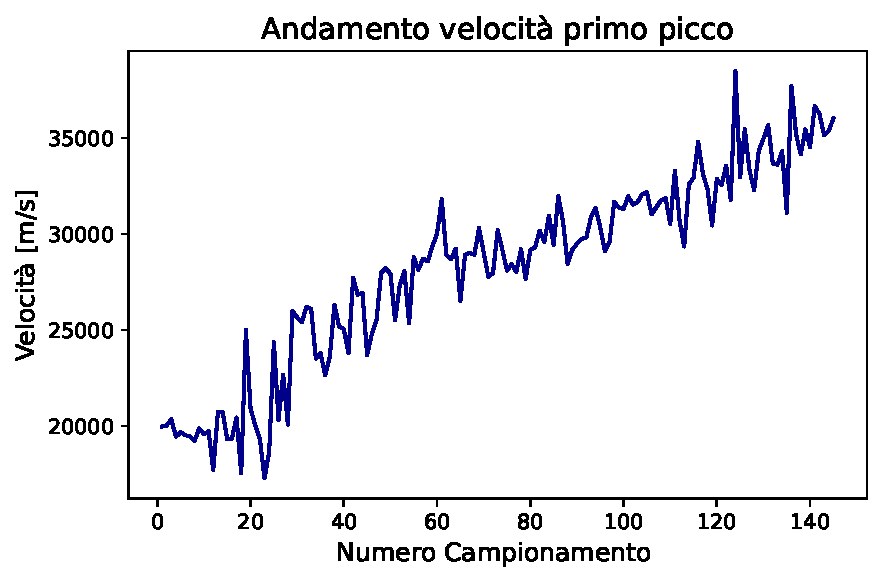
\includegraphics[scale=0.8]{Prima_NO.pdf}
	\caption{Andamento crescente della velocità, del primo picco, all'aumentare del giorno di osservazione}
    	\label{fig:Prima_NO}
\end{figure}


\begin{figure}[H]
\centering

\begin{subfigure}[h!]{0.49\textwidth}
	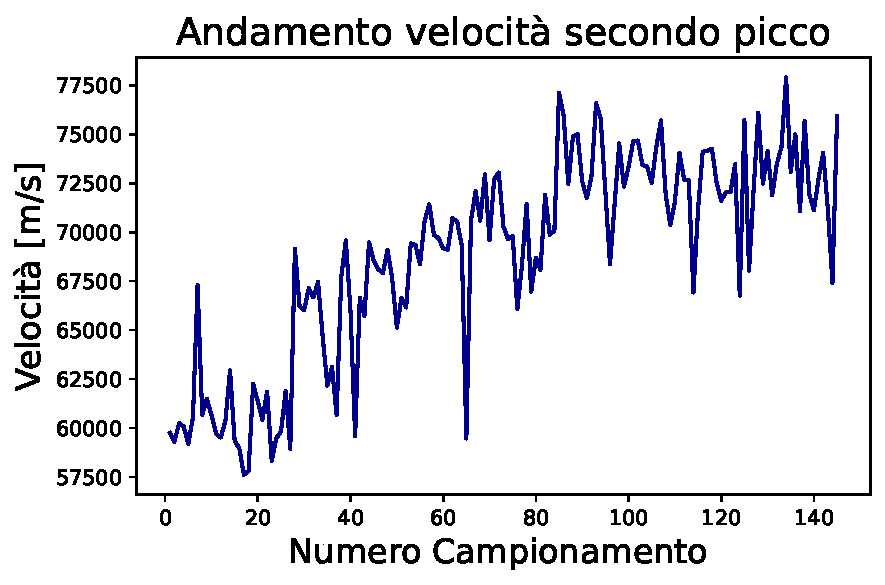
\includegraphics[width=\textwidth]{Seconda_NO.pdf}
    \label{fig:sub1}
\end{subfigure}
\hfill
\begin{subfigure}[h!]{0.49\textwidth}
    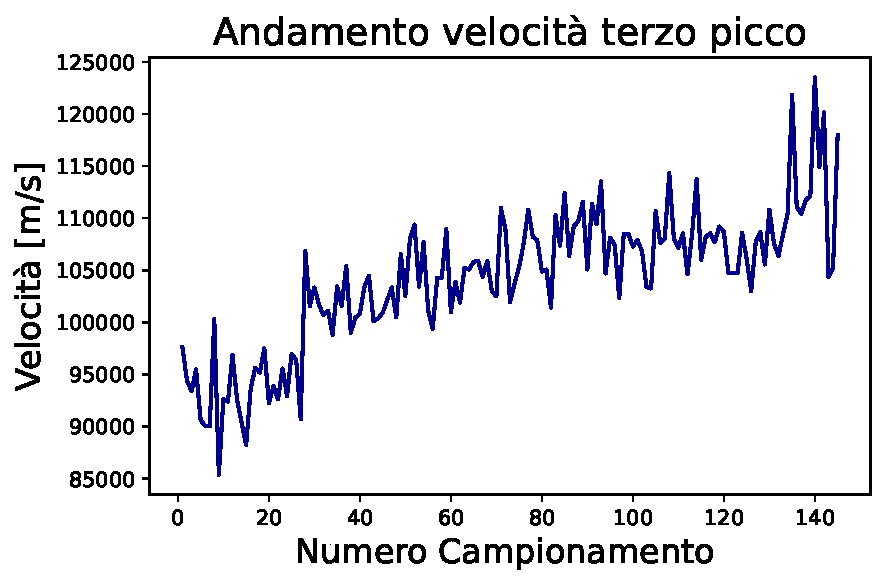
\includegraphics[width=\textwidth]{Terza_NO.pdf}
    \label{fig:sub2}
\end{subfigure}
\caption{Andamenti riferiti rispettivamente al secondo e al terzo picco}
\end{figure}

La correzione è effettuata tenendo conto del moto terrestre. Le velocità ricavate in \ref{Calcolo delle velocità dei tre picchi}, sono dirette lungo la congiungente Terra-Sorgente. Per proiettare la velocità di rivoluzione, della Terra rispetto al Sole, bisogna porsi nello stesso sistema di riferimento. Il sistema scelto è l'HEE, $Heliocentric Earth Ecliptic$, avente come centro il Sole e come asse x la congiungente Terra-Sole. Partendo dalle coordinate, ascensione retta e declinazione, della regione del cigno, e dalla sua distanza $\sim 165435.17  au (astronoic units)$, valore scelto tra il Sole e Deneb, stella più brillante della costellazione; vengono ricavati i valori di latitudine e longitudine, relativi ad ogni giorno di osservazione. Il valore della latitudine è costante, quello della longitudine varia di 30 deg nell'arco di un mese. Tale cambio di coordinate è eseguito ricorrendo alla funzione $coord-celestial.transform-to(HeliocentricEarthEcliptic$, presente nella libreria $sunpy$ \cite{Sunpy:sunpy_community2020}.
\\\\
La velocità finale è calcolata nel modo seguente: 
\begin{equation}
	v_{finale}=v_{picco}-v_{Terra}cos(\alpha)cos(\beta)
\end{equation}

con la seguente notazione, $v_{finale} $ velocità a cui è stata applicata la correzione, $v_{picco} $ velocità del picco senza correzione, $v_{Terra}$ = velocità di rivoluzione della Terra pari a 29780.5556 m/s, $\alpha$ angolo di latitudine, $\beta$ angolo di longitudine.
\\\\
Vengono graficati nuovamente i valori delle velocità in funzione del momento di osservazione, si può notare un andamento oscillante intorno a un valore medio, senza una crescita lungo i mesi di osservazione. 

\begin{figure}[H]
	\centering
	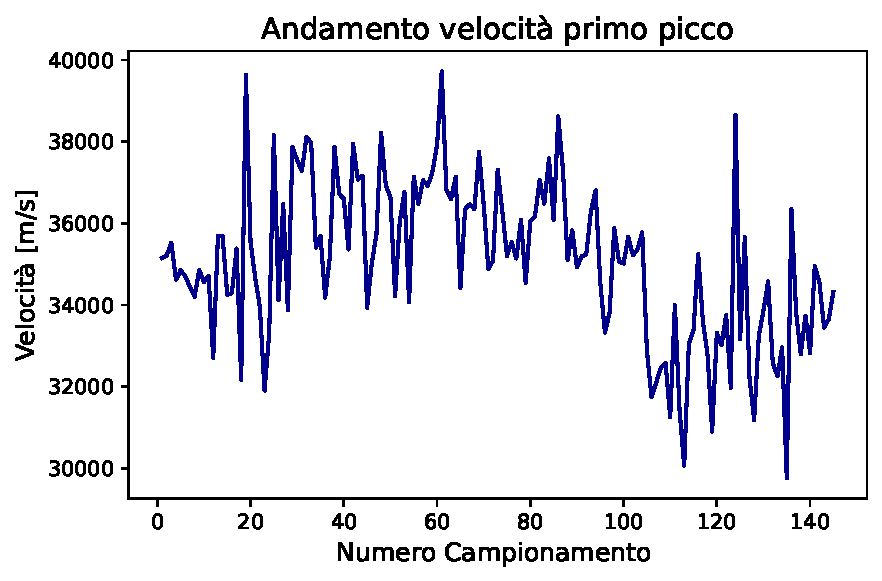
\includegraphics[scale=0.8]{Prima_SI.pdf}
	\caption{Andamento costante della velocità, del primo picco, al variare del giorno di osservazione}
    	\label{fig:Prima_NO}
\end{figure}


\begin{figure}[H]
\centering

\begin{subfigure}[h!]{0.49\textwidth}
	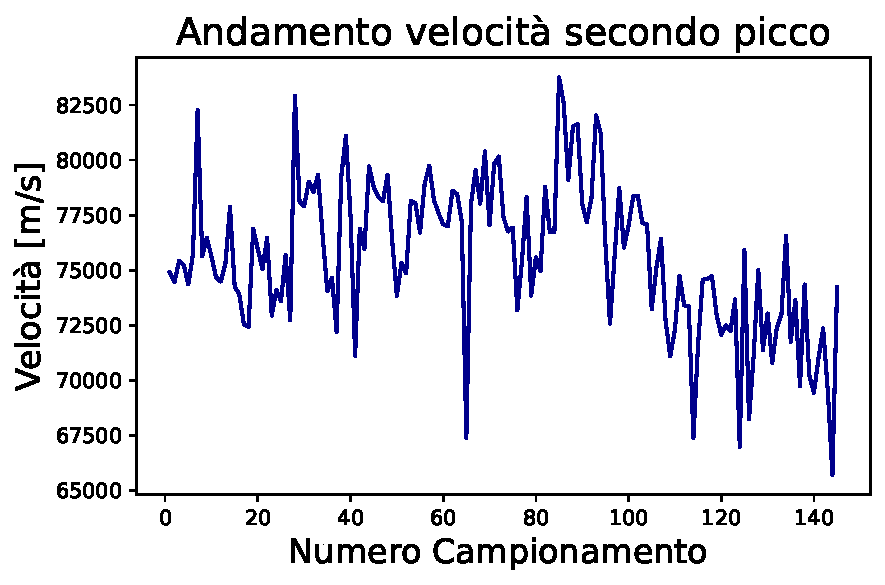
\includegraphics[width=\textwidth]{Seconda_SI.pdf}
    \label{fig:sub1}
\end{subfigure}
\hfill
\begin{subfigure}[h!]{0.49\textwidth}
    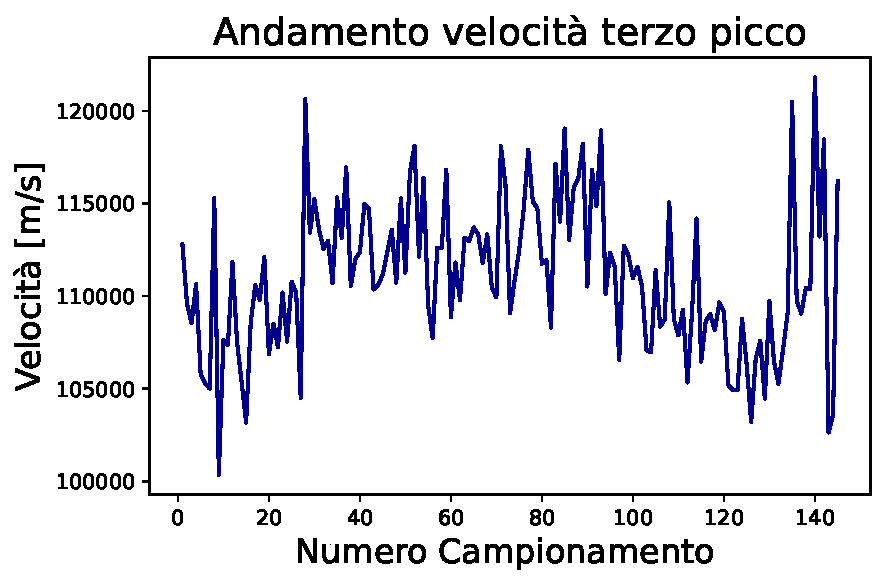
\includegraphics[width=\textwidth]{Terza_SI.pdf}
    \label{fig:sub2}
\end{subfigure}
\caption{Andamenti riferiti rispettivamente al secondo e al terzo picco}
\end{figure}


\subsubsection{Dispersione delle velocità}

Per ottenere il valore di velocità media e relativa dispersione, per ogni picco, i set di valori vengono posti in un istogramma e successivamente fittati gaussianamente. Vengono riportati i risultati finali con i rispettivi grafici:

	

\begin{figure}[H]
\centering

\begin{subfigure}[h!]{0.49\textwidth}
	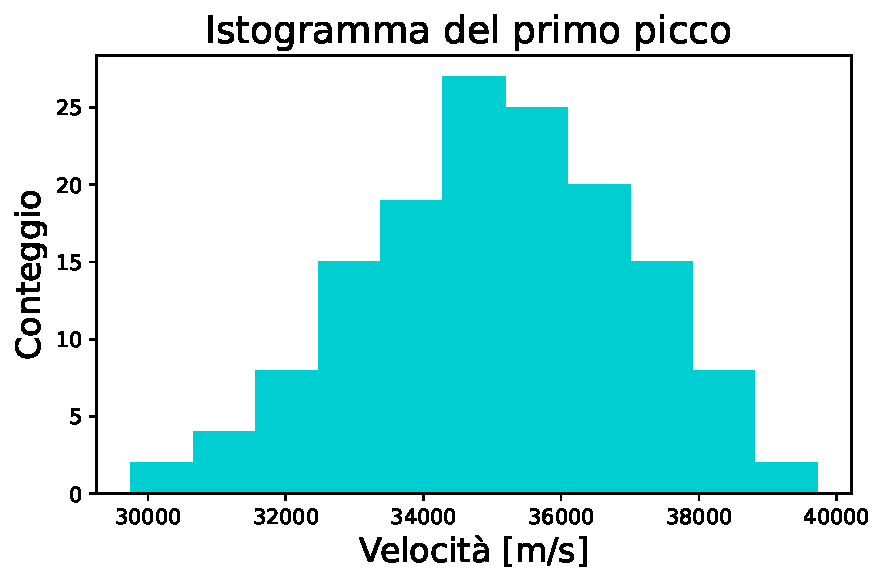
\includegraphics[width=\textwidth]{Primo_histo.pdf}
    \label{fig:sub1}
\end{subfigure}
\hfill
\begin{subfigure}[h!]{0.49\textwidth}
    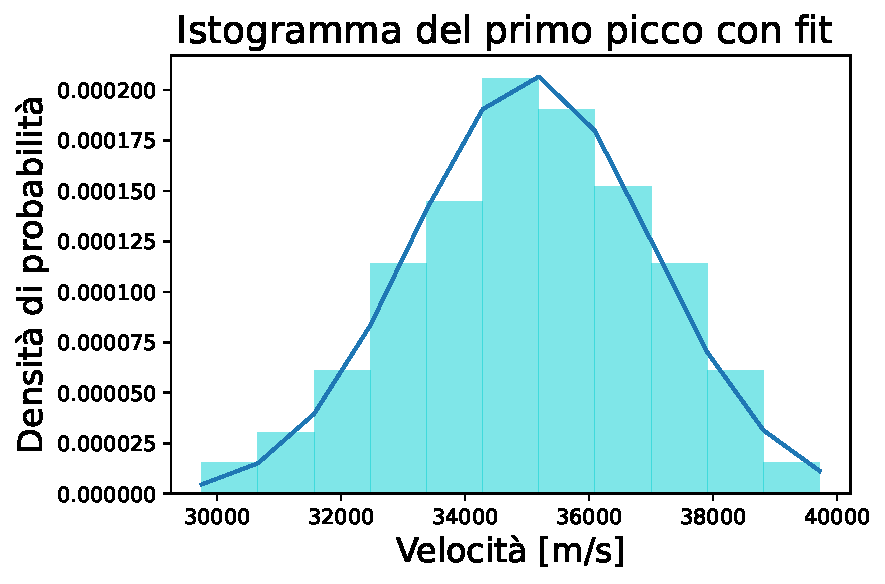
\includegraphics[width=\textwidth]{Primo_histo_fit.pdf}
    \label{fig:sub2}
\end{subfigure}
\caption{Istogramma e fit primo picco}
\end{figure}

\begin{figure}[H]
\centering

\begin{subfigure}[h!]{0.49\textwidth}
	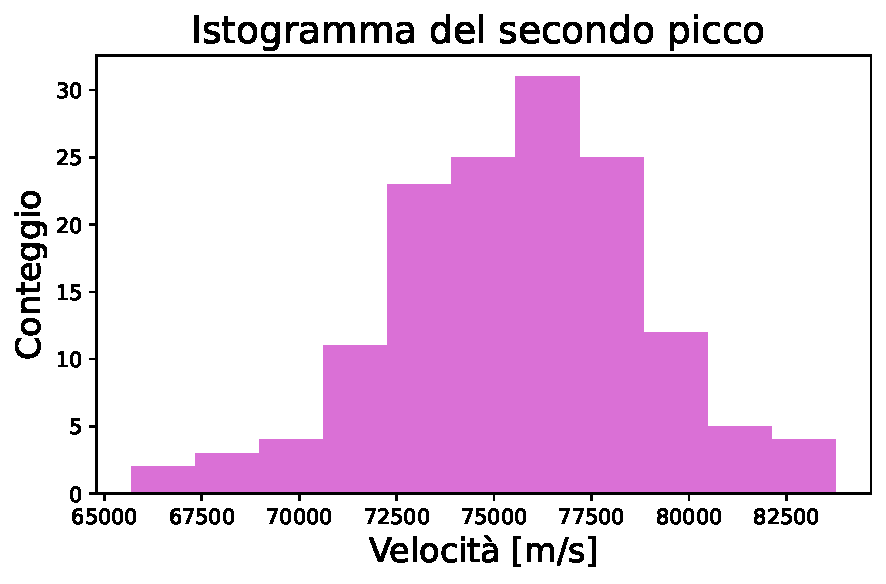
\includegraphics[width=\textwidth]{Secondo_histo.pdf}
    \label{fig:sub1}
\end{subfigure}
\hfill
\begin{subfigure}[h!]{0.49\textwidth}
    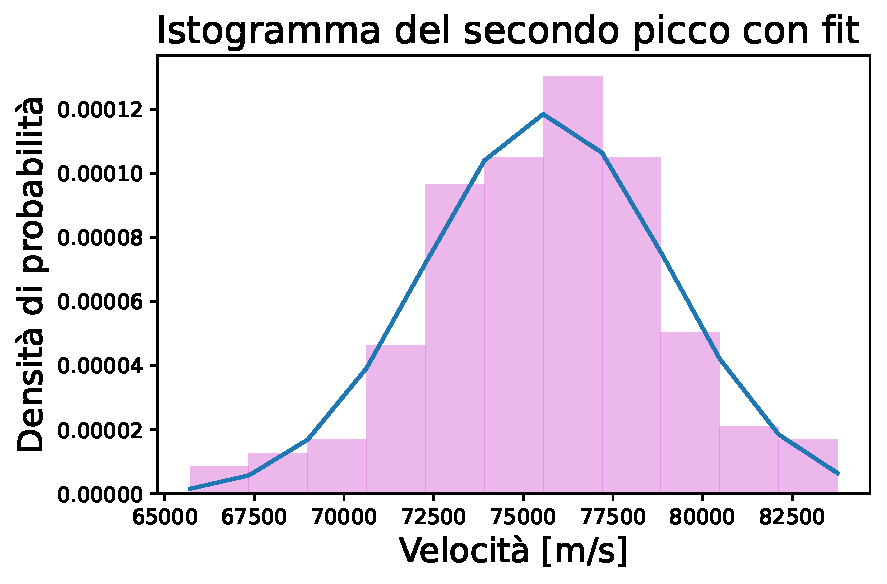
\includegraphics[width=\textwidth]{Secondo_histo_fit.pdf}
    \label{fig:sub2}
\end{subfigure}
\caption{Istogramma e fit secondo picco}
\end{figure}

\begin{figure}[H]
\centering

\begin{subfigure}[h!]{0.49\textwidth}
	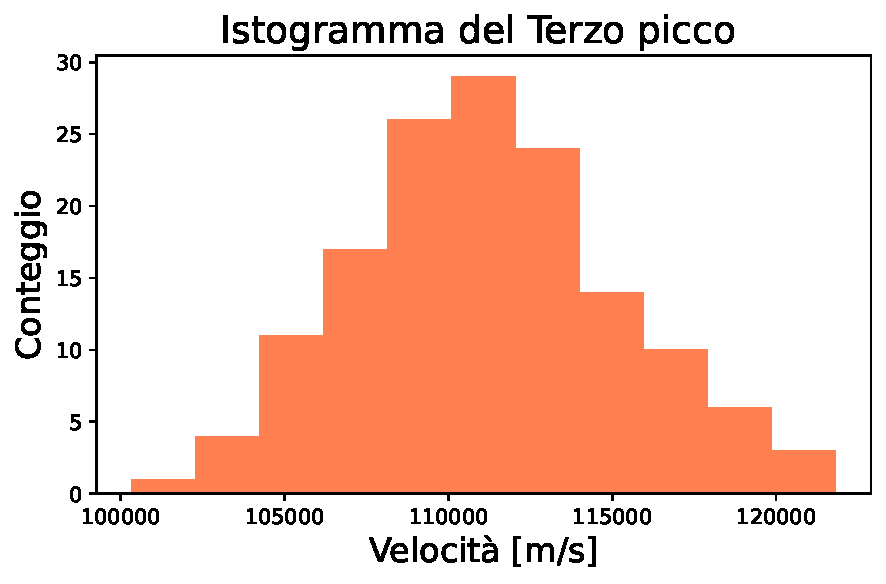
\includegraphics[width=\textwidth]{Terzo_histo.pdf}
    \label{fig:sub1}
\end{subfigure}
\hfill
\begin{subfigure}[h!]{0.49\textwidth}
    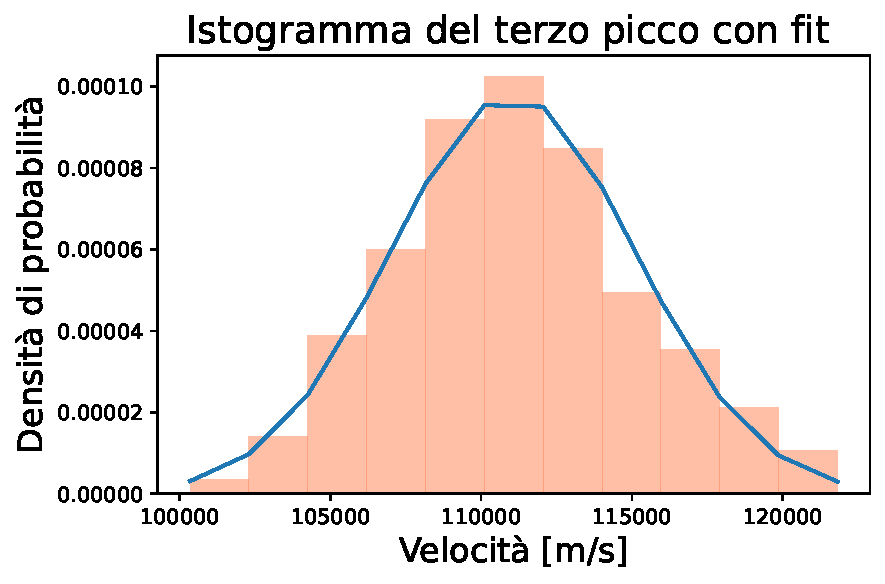
\includegraphics[width=\textwidth]{Terzo_histo_fit.pdf}
    \label{fig:sub2}
\end{subfigure}
\caption{Istogramma e fit terzo picco}
\end{figure}

\begin{table}[H]
\centering

\begin{tabular}{ |c|c|c|  }
	\hline
	\multicolumn{3}{|c|}{Velocità media e deviazione standard} \\
	\hline
	Picco & Vel(m/s)& Dev-std (m/s) \\
	\hline
	Primo &35070,43  & 1926,926    \\
	Secondo &75635,85  & 3365,42  \\
	Terzo &111050,92 &4069,42 \\

	\hline
\end{tabular}

\end{table}

Si osserva, come ci si aspetterebbe, la presenza di tre regioni con velocità diverse, determinando in tal modo tre differenti righe di H 21, discostate ciascuna dal valore teorico per effetto Doppler.



